\subsection{A6 Reporting Student Progress Criterion}

The school leadership and staff regularly assess student progress toward accomplishing the schoolwide learner outcomes and report students’ progress to the rest of the school community.

\subsubsection{Reporting Student Progress}

\indicator{There are effective processes to inform the board, parents, and other stakeholders about student progress toward achieving the academic standards and the schoolwide learner outcomes, i.e., global competencies.}

\prompt{Evaluate the effectiveness of the processes that inform appropriate stakeholders (governing board members, teachers, students, and parents) about student achievement of the academic standards and the schoolwide learner outcomes, i.e., global competencies.}

\begin{findings}
CMIS has multiple processes to inform parents, students, and other stakeholders about student progress. Students and parents are our most important stakeholders, as such, they are provided with many options to keep informed, including: 

\begin{itemize}
\item Biannual family conferences and parent/teachers conferences 
\item Semester Report Cards at elementary
\item \href{https://docs.google.com/a/cmis.ac.th/document/d/1tKgWA7BvpUl5AtPuYD3R3l_bjcqtlilUjVF8mPIiwWA/edit?usp=sharing}{Quarterly Principal Newsletters}
\item As appropriate parent-teacher conferences: formal and informal
\item Bimonthly middle school and high school Communication Groups examine schoolwide learner outcomes and provide teachers with \href{https://docs.google.com/a/cmis.ac.th/presentation/d/1Vivhd6yh4v13MAs9SQlb1j-V6un3hyPROEjYk242zkg/edit?usp=sharing}{student feedback}
\item Monthly community service newsletter: \href{http://blogs.cmis.ac.th/community-service/}{Community Service Student Highlight} to promote global outreach and acknowledge student contributions.
\item Annual ISA, PSAT, and AP report on results to students and parents (MAP results will be available Fall, 2017)
\item Weekly elementary school teacher blogs about due dates, goals, and accomplishments.
\item Anytime parents access student progress in Powerschool  
\item Anytime access to Google Classroom portal for students and parents. 
\item Anytime access to CMIS Facebook page too keep parents and students updated on student initiatives. 
\end{itemize}


\minor{So what...}

The findings indicate that CMIS Leadership and Teaching Staff address this indicator by keeping parents and students updated on the student’s progresses through multiple means. Processes and protocols should be developed to more consistently keep the Board updated on school and student progress and initiatives. 
\end{findings}

\subsubsection{Monitoring of Student Growth}

{\centering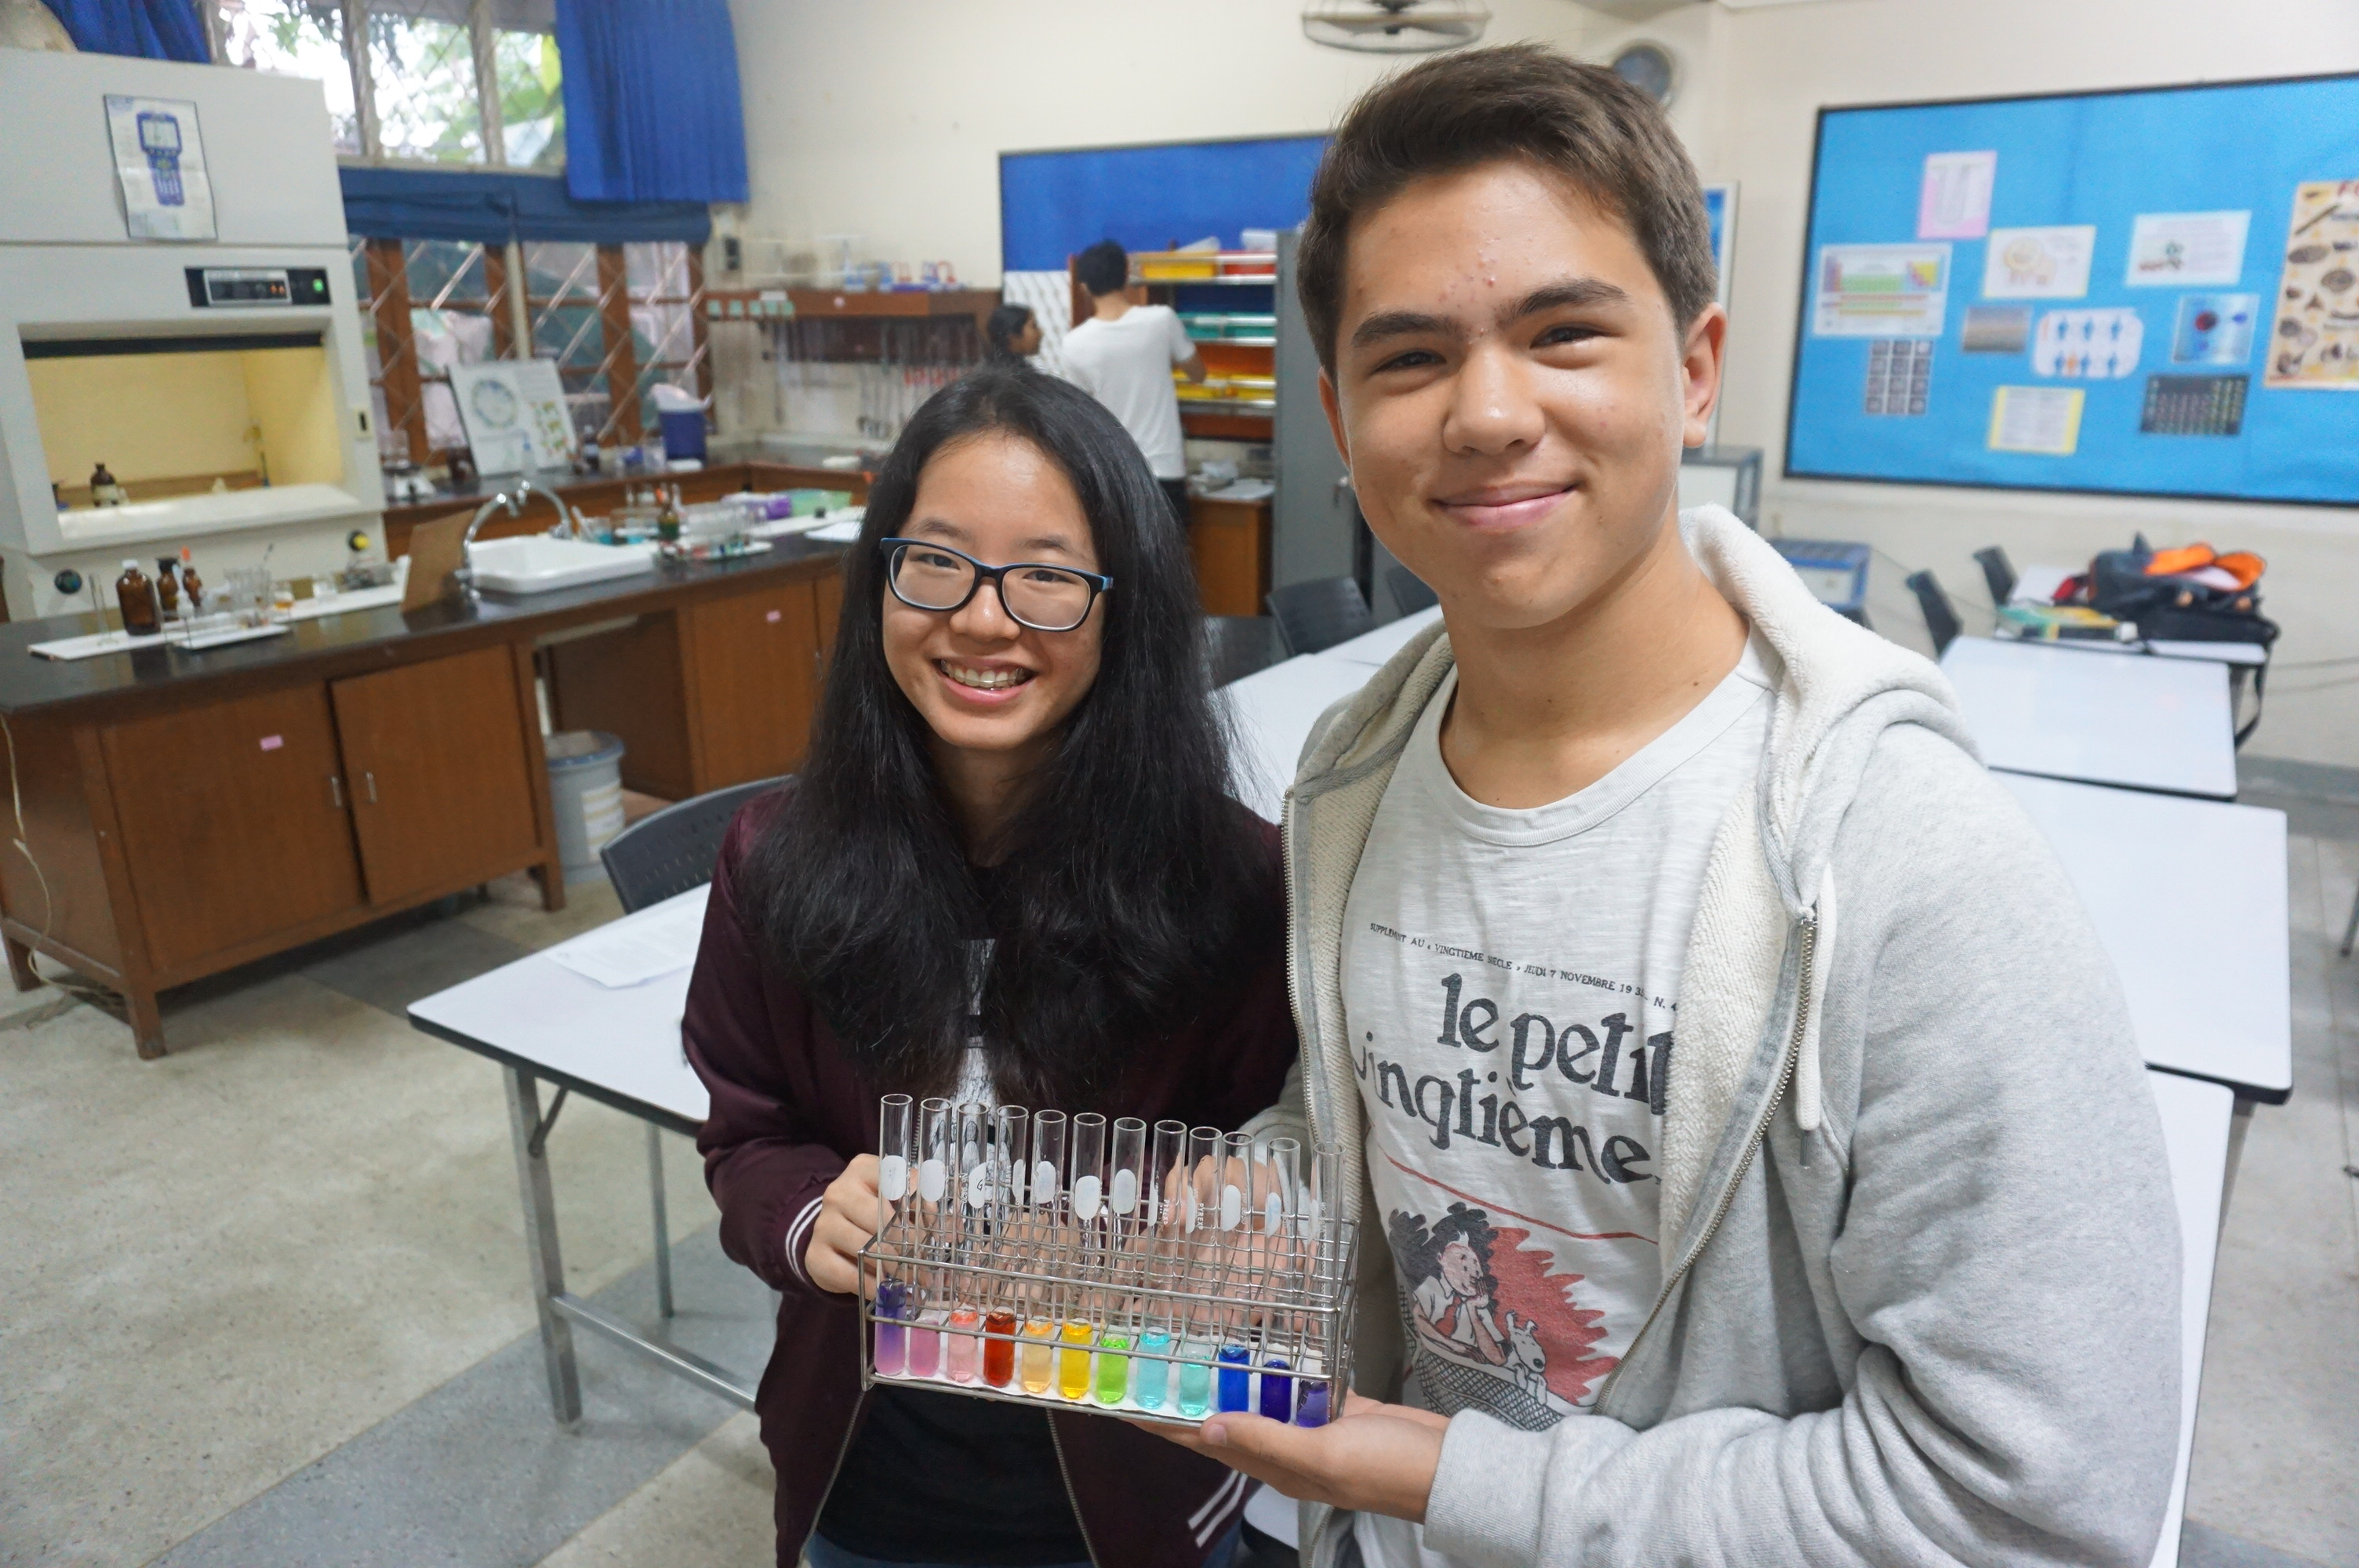
\includegraphics[width=\textwidth]{chapter4_A6.JPG}}

\indicator{The school has an effective system to monitor all students’ progress toward meeting the academic standards and schoolwide learner outcomes.}

\prompt{Evaluate the effectiveness of the system used to monitor the progress of all students toward meeting the academic standards and schoolwide learner outcomes.}

\begin{findings}
CMIS has an effective systems to monitor all students’ progress toward meeting the academic standards and schoolwide learner outcomes.

\minor{Assessment}
 
All K-5 CMIS teachers use the diagnostic assessment, DRA (Developmental Reading Assessment), to help them inform and differentiate their reading instruction. The DRA also progress monitors students throughout the year. 

Many CMIS teachers develop pre assessments specific to their content areas. Teachers use this assessment information to determine where to begin instruction in certain units. 

All CMIS teachers were asked to give the CMIS Common Writing Pre assessment (during the 2015-2016 school year). The pre assessment was used to inform divisional and grade level planning. For example, the common writing pre assessment was used by the English and social studies department to construct a common argumentative rubric using the pre assessments as anchor papers.

ISA and PSAT assessments provide CMIS Leadership, Teachers, and Students norm referenced progress information. Starting in Spring, 2017, CMIS will introduce the MAP norm referenced assessment, in lieu of the ISA, to more rigorously align to our standards 

Used most regularly, teachers monitor progress through the use of their teacher created or curriculum provided, content specific assessments. CMIS has focused on providing students with quality assessment by providing time and resources for high school teachers to peer review their major tests of the semester. 

Finally, formative assessment has been a consistent topic at CMIS since 2014. Please see the section entitled Planning Processes, Professional Development, Student Understanding of Performance Levels in the How Students Learn section, Acceptable Student Achievement and Accessibility of all Students to Curriculum in the What Students Learn section, and Appropriate Assessment Strategies, Teacher Monitoring, and Student Feedback in the How Assessment is Used for more information about how CMIS uses formative assessment. 

\minor{Datawise}

CMIS Leadership and Teaching Staff have used the Harvard Graduate School of Education’s Datawise process to analyze student data to identify a learner centered problem (LCP) and a problem of practice (POP). This LCP and POP are used to help the staff select a research based instructional strategy that is aligned to the standards and is embedded in our instructional planning  throughout the year. 

\minor{Powerschool}
 
All 6-12 CMIS teachers use the Powerschool online platform to help them monitor their student progress. Teachers have a vast array of reports that can help them monitor student progress including: 

\begin{itemize}
\item Absentee	
\item Attendance Count	
\item Class Attendance Audit
\item Discipline Log	
\item Discipline Summary
\item Grade Count by Teacher	
\item Grades Distribution	
\item Graduation Progress Report 
\item Parental Access Statistics
\item At Risk Students	
\end{itemize}

\minor{Student Success Team}

The SSt meet regularly to discuss students of concern, whether it is academic, spiritual, physical or emotional. As mentioned in the Existing Structures section, if teachers have concerns related to their students they are encouraged to reach out to the Student Success Team facilitated by our Student Service Coordinator. There is a Student Service Request Form available on the teacher dashboard section of the CMIS Handbook.This form activates immediate support from the divisional counselor to meet with the teacher and create a plan of action.

\minor{So what...}

CMIS provides many processes and instruments to monitor student progress. Determining whether these processes and instruments are effective should be the next phase in the process. 
\end{findings}

\subsubsection{Modifications Based on Assessment Results}

\indicator{The school uses assessment results to make changes in the school program, professional development activities, and resource allocations demonstrating a results-driven continuous process.}

\prompt{Comment on how assessment results have caused changes in the school program, professional development activities, and/or resource allocations demonstrating a results-driven continuous process.}

\begin{findings}
CMIS uses assessment results to make changes to the school program, professional development activities, and resource allocations demonstrating a results-driven continuous process.
Examples:

In 2014  student data (ISA)  indicated that some of our students were having difficulty in writing, especially organization. In 2015 the Data Wise Process was implemented K-12 and using this data, each department developed a writing framework to improve writing in their grade level.

In 2016 student data (writing samples) indicated that some students had improved in their writing organization but it was difficult to be conclusive as departments were using different assessment formats. All departments are currently working on common assessment and grading practices to help address this need. 

At the beginning of the 2016-17 school year all parents were sent a \href{https://docs.google.com/a/cmis.ac.th/document/d/15NgGowXXl_-_PW3vi8Al-8O8ibZQfgWht9ywRgfjjCY/edit?usp=sharing}{questionnaire} from PTG that asked them to indicate concerns they had about their child’s learning. The Superintendent worked with the PTG Leadership team to use the compiled data to create an annual plan for topics at the monthly PTG meetings.

In 2016 the (\href{https://docs.google.com/a/cmis.ac.th/document/d/14nhwcw8xo3i-23Q-WUxo6KJ_c8yFKu-jTdCctt4MFcs/edit?usp=sharing}{TACT}) process indicated that several staff found the CMIS Faculty Handbook cumbersome. The administration  is currently working with team leaders to modify the format and condense the information to make it a more effective reference tool for staff. 

In 2015 a \href{https://docs.google.com/a/cmis.ac.th/document/d/1hh1nLUlJgg1hd7s6aG3u3We0L6o7Wg_ECdjc2f6DcT8/edit?usp=sharing}{Curriculum Review Cycle} was implemented to resulted in the adoption of Math and Science resources for K-12 standards based instruction.

\minor{So what...}

CMIS regularly uses assessment results to make changes in the school program, professional development activities, and resource allocations demonstrating a results-driven continuous process.There is currently no K-12 standardized tests to assess students across grade bands or tracking progress over time. Including standards based student data (e.g. MAPS) should be the next phase in the process.  
\end{findings}

\subsubsection{Conclusions}
The findings suggest that CMIS addresses this criterion to a high degree. In an effort to increase student achievement further in this area CMIS plans to:

\minor{Maintain and Monitor}

\begin{itemize}
\item Assessment results to make changes in the school program, professional development activities, and resource allocations demonstrating.
\item Ways to seek continual improvement
\end{itemize}

\minor{Investigate Better Practice}

\begin{itemize}
\item Processes and procedures for students to receive standards based feedback. 
\item Processes and procedures to communicate consistent student progress with parents
\end{itemize}



